\documentclass{standalone}
\usepackage{tikz}
\usetikzlibrary{automata,positioning}
\tikzset{
    state/.style={
        circle,
        draw,
        minimum size=20pt,
        inner sep=0pt
    },
    accepting/.style={
        double,
        double distance=2pt
    },
    initial/.style={
        initial by arrow,
        initial distance=7pt,
        initial text={}
    }
}

\begin{document}
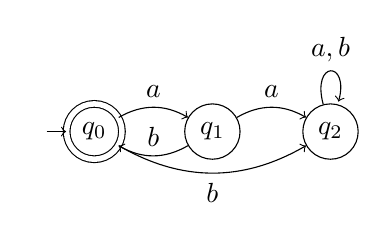
\begin{tikzpicture}[baseline=(current bounding box.center)]
\node[state,initial, accepting] (q0) at (0,0) {$q_0$};
\node[state] (q1) at (1.5,0) {$q_1$};
\node[state] (q2) at (3,0) {$q_2$};
\path[->] 
  (q0) edge[bend left] node[above] {$a$} (q1)
  (q0) edge[bend right, below] node[below] {$b$} (q2)
  (q1) edge[bend left] node[above] {$a$} (q2)
  (q1) edge[bend left, above] node[above] {$b$} (q0);
\path[->]
  (q2) edge[loop above] node {$a,b$} ();
\end{tikzpicture}
\end{document}